% =====================================================================
%  Population genomics of Illex illecebrosus
%  Rewritten 2026-09-18 around the chr2 inversion, its coalescent modelling,
%  and the two-theme (neurodevelopment + photoreception) sweep program.
%  Build:  make            (pdflatex + bibtex)
% =====================================================================
\documentclass[11pt]{article}

\usepackage[utf8]{inputenc}
\usepackage[T1]{fontenc}
\usepackage{lmodern}
\usepackage[margin=1in]{geometry}
\usepackage{graphicx}
\usepackage{booktabs}
\usepackage{amsmath}
\usepackage{amssymb}
\usepackage{textcomp}
\usepackage{authblk}
\usepackage[round]{natbib}
\usepackage{lineno}
\usepackage{xcolor}
\usepackage[colorlinks=true,allcolors=blue,breaklinks=true]{hyperref}
\usepackage{cleveref}

% self-contained: all figures vendored into ./figures/ (portable for GitHub/bioRxiv).
\graphicspath{{figures/}}

\newcommand{\illex}{\textit{Illex illecebrosus}}
\newcommand{\coin}{\textit{I.\ coindetii}}
\newcommand{\Ne}{N_\mathrm{e}}
\newcommand{\Fst}{F_\mathrm{ST}}
\newcommand{\dxy}{d_\mathrm{xy}}

\title{\textbf{A balancing-selected chromosome-2 supergene and a neural and photoreceptive
       program of recent selection in the northern shortfin squid
       \textit{Illex illecebrosus}}}

\author[1,*]{Scott T.\,Small}
\author[1]{Silas B.\,Tittes}
\author[1]{Andrew D.\,Kern}
\affil[1]{Institute of Ecology and Evolution, University of Oregon, Eugene, OR, USA}
\affil[*]{Correspondence: ssmall@uoregon.edu}
\date{Draft \today}

\begin{document}
\maketitle
\linenumbers

% =====================================================================
\begin{abstract}
\noindent
Highly dispersive marine species can show little geographic population structure while
harbouring substantial adaptive genomic variation. Here we use a chromosome-level
reference genome and whole-genome data from 633 northern shortfin squid,
\illex{}, sampled across the Northwest Atlantic to resolve genomic variation that was
previously inaccessible using a divergent reference assembly. We confirm essentially
complete range-wide panmixia, but identify a single major axis of genomic structure:
a $\sim$19~Mb inversion on chromosome~2. The derived arrangement segregates at a
frequency of 0.374, occurs throughout the species' range without a geographic cline,
and reaches $\Fst=0.37$ between alternative homozygotes despite geographic
$\Fst\approx0$. Its evolutionary history is inconsistent with neutral drift. The
rarer derived arrangement retains 2.3-fold more diversity than expected from its
present frequency, and barrier-aware coalescent modelling dates the polymorphism to
$\sim$850~ka, reconstructing a prolonged period near frequency $p\approx0.74$
followed by an active decline over the last $\sim$50--100~ky. The inversion is
gene-poor and lacks functional enrichment, but contains thousands of near-fixed
differences concentrated across the non-recombining block, supporting selection on
the arrangement as a long-lived supergene rather than on a single locally adaptive
locus.

Outside the inversion, demographic analyses support strong expansion (genome-wide Tajima's $D\approx-2$) to a present effective population size of roughly seven million. A stratified,
cross-method-corroborated scan for recent positive selection identified 662 candidate
sweep windows, including 34 high-confidence regions independently supported by
multiple methods. Sweep-associated genes show strong and background-selection-robust
enrichment for two biological themes: neurodevelopment and photoreception, with
additional candidates involving lineage-specific genes and Z-linked RNA-regulatory
and hormone-signalling loci. Together, these results reveal two contrasting modes of
adaptation in an otherwise panmictic marine species: a long-lived chromosomal
polymorphism maintained by balancing selection and recent directional selection on
sensory and neural functions. More broadly, they demonstrate how a conspecific
reference genome can expose structural and adaptive variation that is largely
invisible to geographic differentiation alone.
\end{abstract}

% =====================================================================
\section{Introduction}

Marine populations with enormous census sizes and high dispersal present a persistent
problem for population genetics: weak geographic differentiation can coexist with
substantial evolutionarily important variation that is invisible to conventional
population-structure analyses. This problem is especially acute in pelagic cephalopods.
Ommastrephid squids are short-lived, semelparous, highly fecund, and capable of extensive
dispersal during both early life and adulthood, producing large and often highly variable
populations whose abundance is closely coupled to oceanographic conditions
\citep{odor1998,arkhipkin2015}. The northern shortfin squid \illex{} exemplifies this
life history. It is an annual, semelparous broadcast spawner distributed across more than
2{,}500~km of the Northwest Atlantic shelf and slope, from the Mid-Atlantic Bight to
Newfoundland and Labrador, where it supports major commercial fisheries in both U.S. and
Canadian waters \citep{odor1998,arkhipkin2015,baker2025}. Recruitment and distribution
are strongly influenced by transport in the Gulf Stream and associated shelf and slope circulation, while adults undertake extensive horizontal and diel vertical migrations.
Together, high dispersal, extreme fecundity, and large population size predict little
persistent geographic structure even while providing abundant substrate for natural
selection.

These same characteristics complicate genomic inference. The fecundity-with-high-mortality
demography of \illex{} is the profile that motivates sweepstakes-reproductive-success
models, in which a small and variable fraction of adults contributes disproportionately
to each generation \citep{hedgecock2011,eldon2006,arnason2023}. Large effective population size can
simultaneously increase the efficacy of weak selection, preserve abundant standing
variation, and generate very short linkage disequilibrium, making population history and
recent selection difficult to disentangle. More generally, genomic analysis of
cephalopods has lagged behind that of many commercially important vertebrates because
their genomes are large, repeat rich, and extensively reorganised relative to other
molluscs \citep{albertin2015,albertin2022,schmidbaur2022,coffing2025,coffing2026}. Until recently, these
limitations were particularly severe for \illex{}, for which no conspecific
chromosome-level reference genome was available.

The first range-wide population-genomic analysis of \illex{} provided a critical
baseline. Using whole-genome data from 540 specimens collected across more than 40 sites,
\citet{baker2025} found essentially no geographic genetic structure across the species'
Northwest Atlantic range, consistent with extensive connectivity mediated by early-life
dispersal and adult migration. That study consequently supported treatment of \illex{}
as a single, highly connected stock. However, in the absence of a conspecific assembly,
reads were mapped to the chromosome-level genome of the distantly related diamondback
squid \textit{Thysanoteuthis rhombus}, approximately 51 million years divergent, with a
mean alignment rate of only $\sim$46\%. Such divergence necessarily restricts inference
to the fraction of the genome sufficiently conserved to map reliably and reduces power
in precisely the regions most likely to contain lineage-specific sequence, structural
polymorphism, and rapidly evolving loci. Baker et al. therefore found no evidence of
large structural variants, but explicitly identified reference divergence as a limitation
on their ability to detect them.

Chromosomal inversions are particularly susceptible to this problem because their
evolutionary importance derives not simply from their breakpoints but from the long
haplotypes they maintain. Inversions suppress recombination between alternative
arrangements and can thereby preserve combinations of alleles as segregating
``supergenes'' \citep{kirkpatrick2010,schwander2014,thompson2014,wellenreuther2018,
faria2019}. Many of the best-characterised examples have conspicuous phenotypic effects
or occur in spatially structured populations, including mimicry in \textit{Heliconius}
\citep{jay2021}, alternative reproductive morphs in the ruff \citep{lamichhaney2016},
colony organisation in fire ants \citep{wang2013}, and life-history variation in
\textit{Mimulus} \citep{lowry2010}. Correspondingly, much inversion theory has focused
on local adaptation with migration, where suppressed recombination protects locally
favoured combinations of alleles from gene flow
\citep{kirkpatrick2006,charlesworth2018inv}. Inversions maintained at intermediate frequency without geographic structure pose a different problem. Their persistence
instead implies balancing processes such as overdominance, associative overdominance
generated by recessive deleterious load \citep{zhao2016,gilbert2020,jay2021}, negative
frequency dependence, or temporally fluctuating selection
\citep{wittmann2017,rudman2022}. Distinguishing these histories from neutral drift
requires reconstructing the age and frequency history of the arrangements while
accounting explicitly for the recombination barrier between them
\citep{navarro2000,guerrero2012,berdan2023}.

A chromosome-level \illex{} genome also creates an opportunity to ask where selection
has acted outside large structural polymorphisms. Cephalopods provide an unusual setting
for this question because extreme life history is coupled to exceptional sensory and
neural complexity. Coleoid genomes exhibit substantial lineage-specific reorganisation
\citep{schmidbaur2022}, extensive RNA-editing-based transcriptomic plasticity
\citep{liscovitch2017}, and elaborate nervous and visual systems
\citep{albertin2015,albertin2022,styfhals2022,songcocasey2022}. In squids, vision
operates across large changes in depth and illumination during diel vertical migration,
and photoreception extends beyond the camera eye to dermal opsins and light-responsive
chromatophore systems \citep{mathger2010,ramirez2015,kingston2015}. In a large, highly
connected population where geographic $\Fst$ provides little leverage for detecting
adaptation, recent positive selection should instead be evident primarily through local
distortions of diversity, linkage disequilibrium, and the site-frequency spectrum.
Correctly interpreting those signals, however, requires first establishing the demographic
and genealogical background against which they arose.

Here we use a chromosome-level, annotated reference genome for \illex{} recently made available \citep{small2026} to reanalyse
range-wide whole-genome variation at substantially greater genomic resolution. Our
dataset comprises 633 individuals spanning eleven fishery-management divisions \citep{baker2025}, together with \coin{} \citep{coindetii2025} as an outgroup for divergence-based inference and
\textit{I.\ argentinus} as a recently diverged congener \citep{small2026}. We first test whether the
range-wide panmixia reported by \citet{baker2025} persists when reads are mapped to a
conspecific reference and ask whether previously inaccessible structural variation becomes
apparent. This reveals a single $\sim$19~Mb inversion on chromosome~2 that segregates
across the range despite an otherwise essentially unstructured genome. We then ask
whether this inversion is a neutral polymorphism or a selected supergene by combining
arrangement-specific diversity and divergence with a barrier-aware coalescent model that
reconstructs its age and historical frequency trajectory. In parallel, we infer
population history from the site-frequency spectrum and linkage disequilibrium, explicitly
evaluate whether the data require a multiple-merger rather than Kingman coalescent, and
scan the remaining genome for recent positive selection using complementary methods \citep{kern2018diploshic,alachiotis2018raisd,degiorgio2016}.
These analyses resolve two distinct forms of genomic
adaptation in an otherwise panmictic species: a long-lived, balancing-selected
chromosomal polymorphism and a genome-wide set of recent sweeps concentrated in
neurodevelopmental and photoreceptive functions. Together, they show how a conspecific
genome transforms the apparent genomic landscape of a highly connected marine species,
revealing structural and adaptive variation that is largely invisible to geographic
differentiation alone.


% =====================================================================
\section{Results}

\subsection{Sample, sex, and the absence of geographic structure}
We analysed 633 \illex{} individuals from eleven NAFO management divisions spanning $\sim$37--50$^\circ$N
(\cref{fig:map}, \cref{tab:summary}; every collection event with its source and depth is listed in Supplementary Table~S8). Read coverage on the Z chromosome separates the sample into 342 ZZ
males and 291 ZO females, consistent with a ZZ/ZO system \citep{coffing2025} (\cref{fig:overview}). Autosomal analyses use both sexes; the Z, on which males are diploid and females
haploid, is analysed separately (\cref{sec:sweep}).

Consistent with the range-wide panmixia reported by \citet{baker2025}, population structure exists in
exactly one place in the genome, and that place is not geographic. A
windowed principal-component analysis along chromosome~2 localises the three-cluster structure to the
inversion (among-cluster variance $\eta^{2}=0.748$ inside it against $\eta^{2}=0.003$ in collinear sequence;
Supplementary Fig.~S3), and two genome-wide tests show it is unique. First, the chromosome-2 karyotype
explains none of the variation on any other chromosome (per-chromosome PCA coloured by karyotype:
$\eta^{2}=0.76$ on chr2 versus $\leq0.01$ on all 45 others). Second, and independently of the chr2 labels,
a Gaussian-mixture screen of each chromosome's leading principal component supports more than one cluster
only on chromosome~2 (three clusters, $\Delta\mathrm{BIC}=199$, cluster separation $8.6\sigma$) and on the Z
(two clusters, the expected ZZ/ZO hemizygosity split); every autosome is a single cloud
(\cref{fig:overview}). The residual dispersion on minor PCA axes tracks neither division, latitude, nor
coverage (Supplementary Fig.~S1), and a KING-robust relatedness screen \citep{manichaikul2010} finds no
duplicate, parent-offspring, or full-sib pairs and a single second-degree pair among the 633 individuals
(maximum kinship 0.16), effectively unrelated.
Because a per-SNP differentiation scan is the most sensitive test for local adaptation in a population this
panmictic, we compared per-SNP $\Fst$ among divisions to a coalescent neutral null, a single panmictic population simulated under the fitted demography at the empirical sample sizes and missingness. Across the full per-chromosome callsets of all 633 individuals, thinned to every fiftieth SNP for tractability (551{,}344 autosomal SNPs, those in genes covering 12{,}007 genes), the empirical differentiation lies entirely within the drift expectation: no SNP exceeds the neutral maximum, a single intergenic site passes the lenient threshold against
$\approx$556 expected by chance, and there are zero genic outliers (Supplementary Figs.~S2, S19). Nucleotide
diversity and Tajima's $D$ are flat across latitude and pairwise $\Fst$ among divisions is $\approx0$
throughout (\cref{fig:diversity}). There is therefore no geographic local adaptation anywhere in the genome,
and the inversion itself is geographically non-clinal (\cref{fig:map}; Supplementary Fig.~S6 and Table~S2). Nor does arrangement frequency track capture depth, which spans 3 to 613~m across collection events (Supplementary Table~S8): across 539 individuals with recorded depth the correlation between depth and the number of inverted chromosomes carried is $\rho=-0.08$ ($p=0.08$), and within the six divisions sampled at more than one depth it is $\rho=+0.04$ (within-division permutation $p=0.49$). A weak negative slope across collection events ($p=0.04$) is carried entirely by the two shallow, jig-caught Newfoundland (3K) samples and disappears when they are removed ($p=0.23$), so it cannot be separated from gear and location.

\subsection{A large, balancing-selected inversion on chromosome~2}\label{sec:inv}

\paragraph{Identity, breakpoints, and karyotypes.}
Local PCA \citep{li2019lostruct} and a Gaussian-mixture karyotype assignment (95.3\% confident) resolve three
genotype clusters on chromosome~2 (254 AA, 284 AB, and 95 BB individuals; \cref{fig:inv}a) whose differentiation is karyotypic, not geographic: $\Fst(\mathrm{AA,BB})=0.37$ inside the inversion against a
geographic $\Fst\approx0$. Between-karyotype $\Fst$ computed along the whole chromosome is $\approx0$ (median
0.006) across collinear sequence and jumps to a median of 0.34 (maximum 0.53) inside the inverted body
(Supplementary Fig.~S20), so the karyotypes are one panmictic population everywhere except within the
barrier. The three karyotypes co-occur throughout the range with no latitudinal cline in arrangement
frequency (0.29--0.46 across divisions; \cref{fig:map}; Supplementary Fig.~S6 and Table~S2). Two independent
lines pin the breakpoints to chr2:60.54--79.50~Mb (a $\sim$18.96~Mb differentiated body): a
step-change in arrangement differentiation and a strand flip in a whole-chromosome alignment to \coin{}
(Supplementary Fig.~S11); an extended block of linkage disequilibrium coincides with the same interval
(Supplementary Fig.~S4).

\paragraph{The reference genome carries the derived arrangement.} The derived, inverted arrangement is BB, at a present frequency of 0.374; AA is ancestral and
standard. This is the reverse of the naive polarisation from the reference allele, which is circular because
the \illex{} reference assembly is itself in the inverted orientation (it carries BB at 86.5\% of
fixed-different sites). Restricting to the non-circular subset of sites at which \coin{} carries the \illex{}
alternate allele shows AA to be ancestral (63.0\%) and BB derived: a single inversion event, with the reference simply assembled from an inverted individual (Supplementary Table~S3).

\paragraph{The inversion does not follow a neutral trajectory.}
The primary evidence is per-arrangement diversity (\cref{tab:inv}, \cref{fig:inv}c). Inside an inversion the
two arrangements behave as partially isolated demes \citep{navarro2000,guerrero2012}, so at neutral
equilibrium the diversity of each should scale with its frequency. The rare derived arrangement is instead more diverse than its frequency can sustain: $\pi_I/\pi_S=1.356\pm0.048$ against an equilibrium expectation of $p/(1-p)=0.60$ for a polymorphism held at 0.374, a 2.3-fold excess that is the signature of an old polymorphism that was once common, not of a recent rise. Two diffusion arguments that use neither the mutation rate nor the accessibility mask exclude neutrality (\cref{sec:methods}). The first concerns attainment. A neutral allele must first reach the inferred peak frequency of $\sim$0.74 before it can decline, and the expected time for drift to carry a new mutation to that frequency is $2.1\,\Ne$ generations, which is $\sim$1.15 million generations even at the smallest $\Ne$ on the trajectory (the ancestral $5.5\times10^{5}$), 1.36 times the entire inferred lifetime of the inversion, and up to 17 times at the present $\Ne$; the probability that a new neutral inversion ever reaches 0.74 is of order $10^{-6}$. The second concerns the decline. Over the fitted 100~ky fall, at the $\Ne$ prevailing then ($2.8$--$3.8\times10^{6}$), the standard deviation of allele frequency under pure drift is 0.055, so the observed fall of 0.366 is 6.7 standard deviations of drift; even a fall four times slower would remain 2.5 standard deviations away, and a coalescent profile of the fall duration excludes the slow, drift-compatible alternative at $\Delta\chi^{2}\gtrsim8$--80 (Supplementary Fig.~S14). Both arguments bound drift alone and take the fitted peak frequency as given, but together they establish that the arrangement was neither carried up nor brought down by drift.

\paragraph{Age and frequency history of the inversion.}
Estimating an inversion's age requires a coalescent in which the two arrangements exchange ancestry only
across the barrier; standard simulators do not provide this. We therefore fit the inversion's age and
frequency trajectory with msinv \citep{msinv}, an ancestral-recombination-graph simulator that
enforces the cross-karyotype recombination barrier, tracks ancestral material and outputs tree sequences (\cref{sec:methods}).
The data constrain the shape of the frequency trajectory $p(t)$ rather than any site-level mechanism, so we condition on a deterministic
trajectory under within-arrangement neutrality and fit jointly to $\pi_I/\pi_S$, $\dxy/\pi_I$, and the
per-arrangement singleton spectrum (\cref{fig:demog}b; Supplementary Figs.~S5, S14). The coalescent age is $\sim$850~ky. It is the robustly determined quantity because it is carried by $\dxy$ between
arrangements, which is symmetric to the polarisation. The reconstructed history is that
the inversion arose $\sim$850~ka, coincident with the onset of the population expansion (\cref{sec:demog});
was maintained near $p\approx0.74$ for most of its history; and then fell sharply to 0.374 over
$\sim$50--100~ky, ending $\gtrsim$50--100~ka, under selection of order $\Ne s\sim10^{2}$--$10^{3}$
($s\approx1.5\times10^{-4}$). Simulated inversions of 37~kb rescaled to the 19-Mb body reproduce these
statistics with length-invariance verified over a 25-fold range, and the fitted model reproduces the
observed joint two-dimensional site-frequency spectrum between arrangements, with near-fixed differences and off-diagonal density in the inverted body and a collapse to the diagonal in collinear controls (Supplementary Fig.~S5). Every absolute age scales inversely with the assumed mutation rate $\mu=3\times10^{-9}$, which is the weakest external input to these estimates.

\paragraph{What the inversion is not.} It is not a region of locally suppressed crossing-over. The LD-based recombination map does not register the inversion at all: the estimated rate inside the inverted body equals that of the collinear flanks (medians 0.2015 and 0.2023~cM/Mb), and chromosome~2 as a whole is an ordinary autosome (median 0.202 against an autosomal median of 0.200, the 60th percentile of per-chromosome medians on the same male map; Supplementary Fig.~S12). This is what an estimator that reads linkage disequilibrium in $\sim$19-kb windows should do, because within each arrangement recombination is normal and the barrier operates only between arrangements at the scale of the whole 19-Mb block. The barrier is instead demonstrated directly by the arrangement differentiation, the coincident LD block, and the joint site-frequency spectrum (\cref{fig:inv}b; Supplementary Figs.~S4, S5), and the differentiation is therefore a consequence of the arrangement barrier rather than of a local crossover cold spot. It is not locally adaptive, since there is no cline and geographic $\Fst\approx0$, and the migration-selection scenario that explains most well-studied inversions \citep{kirkpatrick2006} cannot apply. And it is not a swept region, because the genome-wide scan below finds no cross-method-concordant sweep on chromosome~2: the RAiSD footprint statistic is broadly elevated and the classifier over-calls across the inversion, but the two never co-localise into focal concordance, as expected for a balancing-selected supergene rather than a swept locus, and the concordance requirement filters these calls correctly.
Gene flux between arrangements is not detectable in mean $\dxy$, though a residual $\sim$40\% depletion of
near-fixed differences appears in the outermost megabase around the breakpoints. The mechanism of
balancing selection, i.e., overdominance, associative overdominance, frequency dependence, or a moving optimum
under fluctuating selection, is not resolved by these data. Though probable that a shelf-spawning squid whose paralarvae ride
the Gulf Stream would experience temporally fluctuating selection on $\sim$100~ky glacial cycles, however this remains a hypothesis.

\paragraph{Gene content and the architecture of arrangement divergence.}
The inversion has no functionally significant enrichment, yet it carries the molecular signature of a young, recombination-suppressed supergene. It is gene-poor. Its 89 gene models (4.7 per Mb, against 6.8 per Mb genome-wide) place it at the 15th percentile of autosomal windows of the same size (median 127 genes, interquartile range 100--151), and the same holds for annotated content: 45 genes have a cross-species functional annotation and 29 carry gene-ontology terms, again the 15th percentile (median 49 GO-annotated genes per window). Their functional classes are diverse (lipid metabolism, DNA repair, transcription and splicing, signalling) with no coherent pathway (Supplementary Table~S7). A gene-ontology test of its annotated genes against the genome
returns no enriched terms at FDR$<$0.05, and a permutation null shows this is not a power artefact: random gene sets of the same size produce more nominal hits than the inversion genes (86.6$\pm$60 vs 69; permutation $p=0.51$), and the largest nominal per-term enrichments ($\sim$40-fold) rest on as few as two genes (Supplementary Fig.~S21).
The inversion has thus captured a functionally unremarkable slice of the genome,
not a selected gene set but a supergene maintained for the arrangement as a whole. What the
arrangements do accumulate is divergence-as-a-unit: 3{,}513 near-fixed differences between AA and BB
(per-arrangement $|\Delta\mathrm{AF}|\geq0.9$) are spread across the inversion (Supplementary Fig.~S5). These are
overwhelmingly non-coding since coding sequence is only $\sim$0.2\% of the region, but the exonic fixed
differences are $\sim$2.3-fold over-represented and clustered. All 19 fall in just nine genes, led by a cytochrome~P450 (\textit{CYP4X1}) and an acidic-repeat protein (four each) and including a phospholipase~A2, the ciliary gene \textit{RPGRIP1L}, and a cysteine-rich venom-like protein. This is the expected architecture of a balancing-selected inversion that recombines with its homologue only rarely, and it is the raw material from which a supergene's mutation load and eventual degeneration are built \citep{jay2021,berdan2023}. We looked for that load directly and did not find it. Among coding sites inside the body, the most differentiated between arrangements are depleted rather than enriched for nonsynonymous (zero-fold degenerate) positions: 45\% of the top 1\% of coding sites by between-arrangement $\Fst$ are zero-fold, against 82\% of all coding sites in the body (odds ratio 0.18, $p=2\times10^{-34}$), and per-transcript divergence between arrangements is unremarkable relative to collinear controls (5 of 95 transcripts exceed the control 95th percentile, as expected by chance; \cref{sec:methods}). Purifying selection therefore still removes deleterious differences between the arrangements, and any recessive load carried by the rarer arrangement is not yet visible as excess nonsynonymous divergence.

\subsection{Demographic history shows an expanding population}\label{sec:demog}
The age and selection estimates above depend on the population's demography and on the coalescent class
being Kingman. Genome-wide, \illex{} shows $\pi\approx0.0093$ and Tajima's $D\approx-2$ in essentially every
window \citep{tajima1989,tajima1989b}, an unambiguous, genome-wide signature of expansion (\cref{tab:demog},
\cref{fig:demog}a, \cref{fig:diversity}). A moments fit to the folded SFS gives growth from an ancestral
$\Ne=$ 547{,}928 to a present $\Ne=$ 6{,}808{,}096 over 769{,}519 generations ($\sim$12-fold; generations
$\approx$ years for this annual species), and this history reproduces both the observed $\pi$ and a full-SFS
Tajima's $D=-1.92$ under forward simulation. Stairway~Plot~2 and GONE2 concur on strong recent expansion to
$\Ne$ in the $1.5$--$1.7\times10^{7}$ range. Because sweepstakes reproduction would mimic expansion by
inflating rare variants \citep{eldon2006,hedgecock2011,eldon2015}, we tested the coalescent class directly: the folded
SFS is fit far better by a Kingman-plus-growth model than by any multiple-merger (Beta) coalescent
\citep{schweinsberg2003} (shape deviation $L_1=0.036$ vs a best-$\alpha$ 0.108), and contemporary $\Ne$
estimates from the SFS and from linkage disequilibrium agree where both are inconsistent with a strong
multiple-merger process. The expansion began $\sim$770~ka, i.e.\ at essentially the same time as the
inversion arose, which places the supergene's origin at the start of the demographic episode that shapes the
whole genome.

\subsection{Genomic context: recombination, background selection, and protein adaptation}
Three further features of the genome set the stage for the sweep scan. Recombination, as estimated by a deep-learning LD-based map, is $\sim$0.20~cM/Mb on the autosomes (median 0.200; Supplementary Fig.~S12). Because the estimator reads linkage disequilibrium it recovers the sex-averaged rate, so heterochiasmy is not identifiable from it. The map is flat with respect to gene content: the rate varies by only $\sim$6\% between windows adjacent to exons and windows $>$100~kb from any exon, unchanged when $\pi$ is held fixed (Supplementary Fig.~S17a), as a crossover rate should be. It is also compressed at chromosome
scale: on chromosome~1 the rolling median spans just 0.17--0.23~cM/Mb, the pericentromeric flanks where
$\pi$ halves show no more than a 5\% dip, and the centromere itself (a 2.5-Mb block that is 80\% repeat and
almost entirely masked) carries no windows (Supplementary Fig.~S22). The pattern is genome-wide: across
all 43 scanned autosomes the chromosome-scale rolling median varies by only 10--41\% of each chromosome's
median, and no chromosome shows a peak more than 25\% above it. The map therefore fixes the genome-wide
mean well but resolves little broad-scale landscape, and ``nearly uniform'' is in part an estimator
ceiling; none of the analyses below depend on fine-scale recombination variation.
Background selection is moderate and gene-density-driven: $\pi$ falls with local coding density
($r=-0.31$; 20--30\% reduction in gene-dense windows) and rises 43\% between exon-adjacent and exon-distant
windows, while recombination does neither (Supplementary Fig.~S17), the classical footprint of linked purifying selection \citep{charlesworth1993,mcvicker2009,charlesworth2021}, organised here by gene density
rather than by the recombination axis. Diversity is also heterogeneous at the megabase scale: 22 blocks of
$\geq$1~Mb on 17 chromosomes carry 2--4$\times$ the chromosome-median $\pi$ with less-negative Tajima's $D$
(e.g.\ chr1:24--31~Mb, $\pi=0.020$; Supplementary Fig.~S23, Table~S9). Every block is present at the same strength in each of the ten sampling divisions (block-to-flank ratio varying by 1--6\% among divisions), and between-division $\Fst$ is no higher inside the blocks than outside, so none is a regional or population-specific feature (Supplementary Fig.~S23). We tested these against every structural
explanation and they fail all of them: local PCA finds no karyotype clusters (unlike the chr2 positive
control), there is no heterozygosity excess, no excess-heterozygosity filtering loss, and no per-individual
depth anomaly, and their allele-frequency spectrum is identical to flanking sequence; they simply carry $\sim$2.5$\times$ more SNPs. They are gene-poor (coding fraction 0.001), largely unalignable to \coin{}
(35\% vs $\sim$88\% of bases aligned) and 1.7-fold more divergent where alignable, and low-coverage
\textit{I.\ argentinus} reads also call $\sim$3$\times$ more variants in them. They are therefore
fast-evolving, largely lineage-specific gene deserts, shaped by elevated mutation input and relaxed linked selection, not structural polymorphisms, and the chromosome-2 inversion remains the genome's only segregating
karyotype. A model-based $B$-map could not be fit under this
regime (the classical approximation overflows where the deleterious mutation rate exceeds the selection
coefficient), so local coding fraction serves as the background-selection covariate that the sweep scan
controls for explicitly. Protein adaptation over the divergence timescale is substantial:
McDonald--Kreitman tests \citep{mcdonald1991,messer2013mk} against \coin{} across 20{,}999 genes give a
genome-wide proportion of adaptive substitutions $\alpha\approx0.34$--0.64, with the splicing factor
\textit{SF3B4} the single most significantly adaptive gene (Supplementary Fig.~S10). Per-gene power is limited,
so we treat the MK results as complementary to the recent-sweep scan, which detects a different timescale of selection, recent and often non-coding. \textit{I.\ argentinus} is a striking comparator: recently
diverged (an order of magnitude fewer fixed coding differences than \coin{}; Supplementary Table~S3), it
carries near-identical genome-wide diversity ($\pi=0.0092$ vs 0.0093, within 1\%): two large-$\Ne$, expansion-shaped congeners of matched standing variation.

\subsection{A genome-wide scan for selective sweeps}\label{sec:sweep}
We scanned for recent positive selection with diploS/HIC \citep{schrider2016,kern2018diploshic}, a five-class
site-frequency/diversity-based classifier (neutral, hard, soft, linked-hard, linked-soft; 1.1~Mb feature
windows of eleven 100~kb sub-windows) trained on forward and coalescent simulations under the fitted growth
demography (\cref{fig:selection}; Supplementary Figs.~S7, S8).

\paragraph{The scan must be framed as an outlier detector.}
Two methodological findings shape everything that follows. First, a training/scanning feature mismatch, in which the model was initially trained on phased-haplotype simulation features but applied to unphased genotypes, inflated linkage-based features by an order of magnitude and had to be corrected by retraining on the same
unphased feature extractor used to scan; the final full-SFS model reaches 81\% class accuracy
(Supplementary Fig.~S7). Second, and more fundamentally, even the corrected model over-calls sweeps on the real genome: real neutral windows (accessible, $\geq$5~kb from any gene) carry 3--8-fold more
within-window spatial heterogeneity in $\pi$ and $\theta$ than the simulations, even though their marginal
SFS matches ($D\approx-2$). We ruled out missing-data structure and sample incompleteness as the cause; the
residual is real per-sub-window diversity variation (mutation-rate variation plus background selection) that
a uniform-$\theta$ coalescent does not reproduce, a concrete instance of the simulation-to-reality gap
that current best-practice guidance warns against \citep{johri2022}. We therefore use the classifier as a stratified empirical-outlier detector: the sweep score ($p_\mathrm{hard}+p_\mathrm{soft}$) is ranked
within strata of callable fraction and coding density, so a window is an outlier only relative to windows of
similar accessibility and gene density, and calls are corroborated by an independent LD-footprint method
(RAiSD; \citealt{alachiotis2018raisd}) or a composite-likelihood SFS method (SweepFinder2;
\citealt{nielsen2005,degiorgio2016}). We also show that an inherited minor-allele-frequency filter was a
mistake under strong expansion (it discards the rare-variant excess that carries both the expansion and the
sweep signal) and use the full spectrum on both the simulation and empirical sides.

\paragraph{Two tiers of sweep calls.}
We report sweeps at two levels of stringency (Supplementary Fig.~S13). Tier~1 is the diploS/HIC hard/soft classification, spatially resolved by a recombination-aware Markov decoder, a hidden Markov model over the per-window (100~kb) classes with neutral, linked, and sweep-centre states whose emissions are the
prior-corrected class posteriors and whose dwell lengths follow the $\sim$400~kb sweep footprint scaled by
the recombination map (Supplementary Fig.~S13a). Because the genome reads as $\sim$91\% linked-selected under strong expansion, the
decoder's role is spatial coherence: it retains hard/soft calls that lie in contiguous sweep centres and
discards spatially isolated ones, reducing 1{,}758 raw calls to 717 windows (658 localised autosomal calls;
459 hard, 199 soft) and preferentially keeping the higher-outlier windows (median empirical-outlier
percentile 0.98 vs 0.95 for discarded calls; Supplementary Fig.~S13b). Tier~2 is the subset
independently corroborated by a footprint method: the 34 cross-method-concordant regions (a diploS/HIC-HMM
outlier plus RAiSD or SweepFinder2). The two tiers agree strongly: 89\% of windows at concordant loci are
decoded as sweep centres versus 2.9\% genome-wide (odds ratio 282, $p<10^{-46}$), and 30 of the 34 concordant
regions contain a Tier-1 centre (Supplementary Fig.~S13c), so the conservative concordance set is a
high-purity subset of the classifier calls, not a disjoint list. Because the decoder could not be
simulation-calibrated at this genome's recombination density (\cref{sec:methods}), its dwell parameters are
set from the sweep footprint and the recombination map and validated post hoc by this concordance; we treat
Tier~1 as a ranked candidate set and Tier~2 as the high-confidence calls. The Z chromosome, which the
footprint methods do not cover, is necessarily diploS/HIC-only; scanned separately in males (below), it
contributes four further Tier-1 calls, for a genome-wide Tier-1 total of 662 (\cref{fig:selection};
Supplementary Fig.~S18).

\paragraph{Two themes: neurodevelopment and photoreception.}
The 658 autosomal Tier-1 calls overlap 894 genes (476 with GO annotation; one-third of calls fall in
gene-poor, often transposon-rich windows and are excluded). A gene-ontology enrichment against the
annotated-gene background (Fisher's exact test, Benjamini--Hochberg FDR; \citealt{benjamini1995}) returns
124 terms at FDR$<$0.05 (Supplementary Fig.~S15, Table~S4), dominated by neural development (neurogenesis, generation of neurons, neuron development, neuron-projection and cell morphogenesis; 1.5--1.8-fold), together with transcriptional and RNA-regulatory control, and a weaker light-response signal
(response to light stimulus 1.9-fold, response to radiation 1.8-fold). The enrichment is carried by the
hard-sweep calls (99 terms); the disjoint soft-sweep set has none at FDR$<$0.05. The decisive test is
whether these themes are artefacts of background selection, since gene-dense neural loci have lower diversity for reasons unrelated to sweeps. We therefore screened every Tier-1 call with the same per-region
background-selection test used for the concordant set, retaining only calls whose local $\pi$ falls below the
background-selection expectation given flanking coding density. This keeps 291 of the 658 (237 hard, 54
soft), and the enrichment does not merely survive the screen; it sharpens. The BGS-robust set
yields 152 terms at FDR$<$0.05, and every leading term's fold enrichment rises: response to light stimulus
$1.92\!\to\!3.12$ (FDR $2\times10^{-2}\!\to\!1\times10^{-4}$), response to radiation $1.75\!\to\!2.77$
(FDR $3\times10^{-2}\!\to\!2\times10^{-4}$), neuron-projection morphogenesis $1.81\!\to\!2.26$, cell
morphogenesis $1.72\!\to\!2.24$, neuron development $1.59\!\to\!1.97$, generation of neurons
$1.60\!\to\!1.90$, transcription by RNA polymerase~II $1.73\!\to\!2.08$ (Supplementary Fig.~S15). The photoreception signal, the weakest in the full set, becomes the single most enriched theme after the screen,
and its more specific child terms (detection of light stimulus $2.5\!\to\!3.9$, phototransduction
$2.5\!\to\!3.4$) move in the same direction, though with too few genes to reach significance. A shared-gene
enrichment map of the BGS-robust set resolves the same two connected modules, neural
development/morphogenesis and light response, with no third (Supplementary Fig.~S16, Table~S5). Because
background selection can only remove diversity where genes are dense, a signal that grows as gene-dense
false positives are removed is the opposite of what a BGS artefact would produce: the sweep program in
\illex{} is a coherent sensory-and-neural one, and it is real.

\paragraph{Candidate sweeps.}
The Tier-2 concordant regions carry a biologically coherent set of cephalopod-orthologous genes that sit
squarely within these themes (\cref{tab:sweep}; Supplementary Table~S6): the neural/EMT transcription factor
\textit{ZEB2}, the synaptic-vesicle GTPase \textit{Rab3}, the apelin receptor \textit{Aplnr}
(cardiovascular/vasculature signalling), the DNA-damage-response gene \textit{MACROD2}, the phospholipid
synthase \textit{cept1}, and, at a locus the annotation had missed, a ceramide phosphoethanolamine synthase. A per-region background-selection test isolates 11 of these as high-confidence candidates in which
diversity is reduced beyond the background-selection expectation, and fine-scale localisation confirms all 11
as recent sweeps by the sign of Tajima's $D$ at the diversity valley, reassigning two apparent gene-desert
signals to transposable-element regions (flagged lower confidence) and one candidate's target to a neighbouring
gene. The single most distinctive autosomal candidate is a cephalopod-lineage-specific gene under a hard sweep on chromosome~16, a tandem-exon transcript with no functional annotation whose translation matches an uncharacterised protein family in the bobtail squid \textit{Euprymna} ($E=2\times10^{-53}$), the kind of lineage-specific novelty that cephalopod genomes are known to generate
\citep{albertin2015,albertin2022}. There is no overlap between the sweep candidates and the MK-adaptive genes,
as expected for their different timescales.

\paragraph{The Z chromosome.}
Because males are Z-diploid and females Z-haploid, the Z was scanned separately in the 330 confident ZZ
males, using a model retrained at the matched sample size (the classifier's features are sample-size
dependent) and a formal adequacy gate for the Z's reduced effective size; the male-only screen was validated
against the 289 haploid females, whose per-window diversity tracks the males' at $r=0.996$. Of the four Z
Tier-1 calls (three hard, one soft; Supplementary Fig.~S18), three credible, gene-localised sweeps survive
fine-scale triage, all confirmed as conserved cephalopod genes by direct homology: \textit{Pasilla}/Nova-1 (a neuronal alternative-splicing regulator; 92\% identity to \textit{Octopus}), \textit{Smaug}/samd4a (a germline RNA-binding translational repressor), and \textit{Esrrg} (an estrogen-related receptor with an adjacent likely \textit{cis}-regulatory lncRNA; 97.5\% identity to \textit{Octopus}), a coherent
RNA-regulation-and-hormone-signalling signature on the sex chromosome that echoes the neural theme of the
autosomes. The \textit{Amnionless}/``Zfest'' sex-determination locus falls just outside the swept valley and
shows only purifying selection: a linked passenger, not the target.

% =====================================================================
\section{Discussion}

\illex{} emerges as a large-$\Ne$, expansion-dominated genome carrying a single dramatic axis of structure, a balancing-selected chromosome-2 supergene, against an otherwise unstructured, moderately
background-selected background on which recent directional selection has acted on a specific biology. Where
the earlier survey \citep{baker2025} established panmixia for management, our contribution is to find the
inversion beneath it, to explain it, and to look past it.

\paragraph{The inversion is a datable, declining, balancing-selected supergene.}
Most inversions whose evolutionary dynamics are understood are maintained by local adaptation with migration
\citep{kirkpatrick2006,lowry2010,faria2019}; the \illex{} inversion cannot be, because there is no geography to adapt to: arrangement frequency is non-clinal and geographic $\Fst$ is zero everywhere. It must instead
be held by balancing selection, and the data constrain how it has been held with unusual precision.
The excess diversity of the rare derived arrangement forces a history in which BB was once common; two
mutation-rate-free arguments and a barrier-aware coalescent fit converge on an $\sim$850~ky-old polymorphism
that plateaued near 0.74 and has been actively driven down to 0.37 over the last $\sim$50--100~ky. This is a
qualitatively different object from the classic \textit{Drosophila} inversions, whose frequencies track
clines and seasons \citep{corbettdetig2012,kapun2019}, and from the human 17q21 inversion, whose signature is a recent
rise under positive selection \citep{stefansson2005}. It resembles more the mimicry supergene of
\textit{Heliconius numata}, where an inverted arrangement carries a recessive deleterious load that
generates associative overdominance and caps its frequency \citep{jay2021}. Associative overdominance is a
natural candidate here: theory shows it emerges precisely in large, non-recombining blocks once recessive
load accumulates \citep{zhao2016,gilbert2020,berdan2021}, and the clustered coding divergence we document (19 exonic fixed differences in nine genes, in a block whose 45 annotated genes show no functional enrichment) is the raw material of such a load, even though the differentiated coding sites are not yet enriched for nonsynonymous change. But a two-phase history of plateau followed by decline is also what selection toward a shifting
optimum can produce \citep{matuszewski2015}; fluctuating selection is demonstrably strong in wild populations
\citep{wittmann2017,rudman2022}, and a shelf spawner whose
paralarvae are advected by the Gulf Stream is a plausible target of $\sim$100~ky climate cycles. The data
constrain the trajectory, not the mechanism. What they do establish is that the arrangement itself, not any
single gene within it, is the unit of selection: the block is gene-poor, functionally unremarkable,
differentiated as a unit, and free of sweeps, exactly as expected when recombination suppression is the trait
under selection \citep{kirkpatrick2010,berdan2023}.

Two features of the inversion analysis are methodologically general. First, the age is carried by the
polarisation-symmetric divergence between arrangements, so it survived a complete reversal of which arrangement is derived, a reversal forced on us by discovering that the reference genome is itself inverted.
Reference-orientation circularity is a hazard for any inversion study that polarises from the reference
allele, and outgroup-based polarisation on non-reference sites is the remedy. Second, the coalescent inside an
inversion is a two-deme process with a barrier \citep{navarro2000,guerrero2012}, and fitting it requires a
simulator that enforces the barrier in the ancestral recombination graph rather than approximating the
arrangements as freely recombining. msinv provides this, and the plateau-and-decline history it recovers is
not accessible to methods that treat the inversion as a single locus. As the catalogue of wild inversions
grows \citep{wellenreuther2018,merot2020}, joint estimation of age, trajectory and selection from
per-arrangement diversity, divergence and the joint SFS offers a route to classifying them by history rather
than by phenotype.

\paragraph{The sweep program is neural and photoreceptive, and it is robust to background selection.}
The genome-wide scan resolves into two themes. The first, neurogenesis, neuron development, and neuron-projection and cell morphogenesis, is what one might expect of a lineage whose defining evolutionary
innovation is a large, centralised, cell-type-rich nervous system \citep{albertin2015,styfhals2022}, and
whose genomes are marked by regulatory reorganisation around neural genes \citep{schmidbaur2022}. The same signature has now been seen in a second coleoid lineage: in the sibling octopuses \textit{Octopus bimaculatus} and \textit{O.\ bimaculoides}, positive selection is concentrated in genes for brain and eye development \citep{coffing2026}, so neural and visual genes may be a recurrent target of recent selection across cephalopods. The
second, photoreception, is the more surprising and the more \illex{}-specific. Cephalopod photoreception is
not confined to the camera eye: opsins and phototransduction cascades are expressed in skin and
chromatophores \citep{ramirez2015,kingston2015}, and the visual system is highly cell-type-diverse, with optic lobes
elaborated convergently with those of vertebrates \citep{songcocasey2022,styfhals2022,yoshida2015}. \illex{} is a fast,
visually guided predator that migrates vertically each day through a steep light gradient and seasonally
across latitude \citep{odor1998}; selection on light detection is biologically apposite. The decisive
evidence that these themes are real, rather than by-products of reduced diversity at gene-dense neural loci,
is their behaviour under the background-selection screen. Background selection lowers diversity where genes
are dense \citep{charlesworth1993,mcvicker2009,charlesworth2021}; a sweep call that is really a BGS artefact
is therefore removed by a test that demands diversity below the BGS expectation, and any enrichment
riding on such calls should erode. Instead every leading term sharpened (light response $1.9\!\to\!3.1$, radiation $1.8\!\to\!2.8$, morphogenesis $1.7$--$1.8\!\to\!2.2$--$2.3$) and the weakest theme became the strongest. The sweep program is not an artefact of gene density.

We frame these as candidates rather than confirmed targets, and the framework itself is offered as a
contribution. Simulation-trained per-window classifiers are increasingly standard
\citep{schrider2016,kern2018diploshic}, but on a strongly expanding, unphased, missing-data-rich genome they
over-call because real neutral sequence is spatially more heterogeneous than tractable neutral simulations.
Rather than hide this behind a threshold, we quantified it and let it dictate the framing, with a stratified empirical-outlier scan, cross-method concordance, and an explicit background-selection filter, in the spirit of recent calls for inference that models the confounders it cannot remove \citep{johri2022}. The
predominance of hard over soft sweeps in the enriched set is notable because a population this large is
expected to adapt mainly by soft sweeps from standing variation \citep{messer2013soft}; a hard-sweep excess
instead points to strong selection on new or rare variants with a small mutational target
\citep{hermisson2005,harris2018}, in contrast to humans, where soft sweeps appear to dominate
\citep{schrider2017}; the soft-sweep class is underpowered here, however, and we draw no firm conclusion about
the mode of adaptation.

\paragraph{Demography, sweepstakes, and what licenses the rest.}
A sweepstakes-reproduction species is exactly where multiple-merger coalescents are expected to masquerade as
expansion \citep{eldon2006,hedgecock2011}, and recent work on Atlantic cod argues that pervasive recurrent
sweeps can themselves generate multiple-merger genealogies \citep{arnason2023}. We tested the coalescent class
directly rather than assuming it: the SFS is Kingman-plus-growth, not Beta, and SFS- and LD-based $\Ne$ agree.
That result is what licenses every age and selection estimate above, and it means that \illex{}'s enormous
fecundity has not, at the genomic scale we can resolve, translated into the skewed genealogies its life
history would suggest. That the inversion arose at essentially the same time as the expansion began is a
coincidence worth noting: a supergene established at the onset of a $\sim$12-fold demographic expansion
would have been carried through that expansion at its plateau frequency, and its subsequent decline is a
recent event against that backdrop.

% =====================================================================
\section{Limitations}
The callset is unphased, so no haplotype-homozygosity statistics are available; sweep detection relies on the
SFS and diversity alone, which limits power against soft sweeps in particular. The simulation-to-real neutral
mismatch that drives classifier over-calling is real and unresolved at the level of absolute neutral calling; our empirical-outlier framing is a principled response, not a cure, and it also defeats a
within-arrangement SFS approach to the inversion. Every inversion age scales inversely with the mutation rate,
and $\mu=3\times10^{-9}$ is the weakest external input; an independent calibration (e.g.\ a karyotyped
congener such as \textit{I.\ argentinus}) is the clearest route to a mutation-rate-free age. The inversion
model conditions on a deterministic frequency trajectory and within-arrangement neutrality; it constrains the
shape of $p(t)$, not the mechanism of balancing selection. The LD-based recombination map has a compressed
dynamic range at chromosome scale and does not resolve centromeric suppression (Supplementary Fig.~S22);
it is used only for its genome-wide mean and for the decoder's dwell scaling, and the absence of a diversity-recombination relationship in these data should be read with that ceiling in mind. The
corroborating footprint methods are broad, and the recombination-aware decoder is design-informed rather
than simulation-calibrated. Candidate sweep genes
rest on homology to distant cephalopod models and on cross-method concordance; the two enrichment themes are
statements about gene sets, not about individual confirmed targets.

% =====================================================================
\section{Methods}\label{sec:methods}
Full parameter values, software versions, and command-level provenance are in
Supplementary Table~S1 and in the project repository.

\paragraph{Data.}
The ingroup is all 633 \illex{} individuals whole-genome sequenced by \citet{baker2025} (ENA project
PRJEB101095; collected 2022--2023 across eleven NAFO divisions, every individual with coordinates), of which
that study retained 540, excluding 93: 616 passed its genotyping quality filters and a further 76 were removed for $>$25\% missing genotypes, a consequence of the 46\% mean read-alignment rate to the \textit{Thysanoteuthis} reference.
Against the conspecific assembly no individual-level exclusion was needed. We re-processed the raw reads from scratch: mapping to
the \texttt{Illex\_F24} primary assembly (45 numbered chromosomes plus the Z) and joint variant calling
(Supplementary Table~S1). Genotypes are unphased and the VCF
is variants-only (no invariant sites), so diversity is computed from genotype likelihoods off the BAMs rather
than from called genotypes. \coin{} is the divergence/MK outgroup; \textit{I.\ argentinus} is a secondary
comparator. An accessibility mask restricts all analyses to callable sites.

\paragraph{Diversity, SFS, and demography.}
Site-frequency spectra, Watterson's $\theta$, per-window $\pi$ and Tajima's $D$, and per-karyotype spectra
were computed with ANGSD \citep{korneliussen2014angsd} (\texttt{-doSaf}/\texttt{realSFS}); per-population
statistics were computed per NAFO division and per chromosome (all 45 autosomes plus the Z, the latter in
males only). Demographic history was inferred with Stairway~Plot~2 \citep{liu2020stairway}, moments
\citep{jouganous2017moments}, and GONE2 \citep{gone2}, and validated by forward simulation reproducing the
observed $\pi$ and $D$. The coalescent class was tested by comparing the folded SFS against Kingman-plus-growth
and Beta-coalescent expectations. Windowed $\pi$, $\dxy$, $\Fst$, and PCA used pg\_gpu \citep{pggpu};
per-SNP and between-karyotype $\Fst$ used the Hudson estimator \citep{bhatia2013}. Relatedness was screened
with KING-robust \citep{manichaikul2010}.

\paragraph{Karyotyping and the inversion.}
Karyotypes were called by local PCA \citep{li2019lostruct} and a Gaussian-mixture model. Arrangement
polarisation used an AnchorWave \citep{song2022anchorwave} \coin{}$\leftrightarrow$\illex{} whole-genome
alignment restricted to non-reference-biased sites, with est-sfs \citep{keightley2018estsfs} as a check. The
inversion's age and frequency trajectory were fit with msinv v0.3.5 \citep{msinv}, an ARG-based
coalescent simulator that enforces cross-karyotype recombination barriers and outputs tree sequences,
implementing hull-based ancestral-material tracking in the msprime lineage \citep{kelleher2016,baumdicker2022};
it was validated against
SLiM \citep{haller2019slim}, msprime \citep{baumdicker2022}, and discoal \citep{kern2016discoal}. All
coalescent simulations underlying the inversion age and decline inference were generated with msinv, and the
complete chr2-inversion analysis (fitting code, simulation configuration, and every per-analysis output and figure) is housed as a dedicated \illex{} module within the msinv repository (\texttt{files/illex/},
\texttt{results/illex/}). Simulations used the fitted growth demography, $\mu=3\times10^{-9}$, and
$r=1.977\times10^{-9}$; statistics were computed on the differentiated body and rescaled from a 37-kb
simulated inversion with length-invariance verified over a 25-fold range. Breakpoints were pinned by
combining arrangement differentiation with the AnchorWave alignment; missed genes were recovered by DIAMOND
\texttt{blastx} \citep{buchfink2021diamond} against seven cephalopod proteomes, with transposable elements
annotated by Earl~Grey \citep{baril2024earlgrey} and transcripts by StringTie2 \citep{kovaka2019stringtie}.
Fixed differences between arrangements were defined as sites with $|\Delta\mathrm{AF}|\geq0.9$ between AA
($n=254$) and BB ($n=95$) homozygotes; the gene-ontology test of inversion genes used Fisher's exact test
against the genome-wide annotated-gene background in all three ontologies, with a permutation null of 500
random gene sets of equal size. Gene density was compared with all autosomal windows of the inversion's length (18.96~Mb, 0.5-Mb step) using the same gene models. The two drift arguments are diffusion results for an unlinked neutral allele: the expected time for a new neutral mutation to first reach frequency $x$, conditional on reaching it, was evaluated in units of $\Ne$ ($2.107\,\Ne$ at $x=0.74$) at each $\Ne$ along the fitted demography, and the drift standard deviation of allele frequency over the fitted decline was computed as $\sqrt{p(1-p)\,t/(2\Ne)}$ with $\Ne$ taken from the fitted growth model over that interval. The load test stratified coding sites inside the body and in a matched collinear control by codon degeneracy (degenotate zero-fold versus four-fold) and compared the zero-fold fraction in the upper tail of per-site between-arrangement $\Fst$ (genotype-likelihood based, $n=40$ per karyotype) with the region's own coding sites by Fisher's exact test; per-transcript $\dxy$ between arrangements was normalised to its 100-kb window and compared with the distribution across control transcripts.

\paragraph{Recombination map.}
A recombination map was built with ReLERNN \citep{adrion2020relernn}
(SIMULATE$\to$TRAIN$\to$PREDICT$\to$BSCORRECT), dropping individuals with no calls on a chromosome and never
forcing diploid genotype calls.

\paragraph{Selective-sweep scan.}
The classifier was diploS/HIC \citep{kern2018diploshic} (five classes, 1.1~Mb windows of eleven 100~kb
sub-windows, twelve diploid statistics per sub-window), trained on SLiM~5.2 forward simulations
\citep{haller2019slim} (recapitated with msprime; \citealt{kelleher2018,haller2019recap}) and pure-msprime neutral
simulations under the fitted growth demography, at the empirical sample size and with realistic structured
missingness. The model was trained on the same unphased feature extractor (\texttt{fvecVcf}) used to scan, on
the full spectrum (no MAF filter). It was used as a stratified empirical-outlier detector (score
$p_\mathrm{hard}+p_\mathrm{soft}$ ranked within callable-fraction $\times$ coding-density strata), corroborated
by RAiSD \citep{alachiotis2018raisd} and SweepFinder2 \citep{degiorgio2016}. The per-window classifications
were spatially resolved into Tier-1 calls with a recombination-aware hidden Markov model (neutral / linked /
sweep-centre states; emissions are the prior-corrected collapsed class posteriors; dwell lengths set from the
$\sim$400~kb sweep footprint scaled by the ReLERNN sex-averaged map, with a constant-rate fallback on
chromosomes~2 and~42 and the Z). A simulation calibration of the decoder was attempted but proved infeasible:
at $\Ne$-scale recombination the recapitated ancestral recombination graphs carry $\sim$3.4$\times10^{5}$
marginal trees per 2.5~Mb, making tree-sequence genotype ascertainment for a training scan prohibitively slow
($>$2.7~h per segment); the dwell parameters are therefore design-informed and validated post hoc by the 89\%/2.9\% Tier-1 to Tier-2 concordance (Supplementary Fig.~S13). The Z chromosome was scanned in males only
with a model retrained at $n=330$ and passed a comparative feature-adequacy gate, then validated against the
haploid females. Candidate genes were annotated with EnTAP and screened by DIAMOND against cephalopod
proteomes. Gene-ontology enrichment of Tier-1 genes used Fisher's exact test against the annotated-gene
background on the scanned chromosomes with Benjamini--Hochberg FDR \citep{benjamini1995}; the
background-selection screen retained calls whose local $\pi$ fell below the expectation from flanking coding
density ($\hat\pi=0.01059-0.16547\cdot f_\mathrm{CDS}$; standardised residual $\leq-0.3$).

\paragraph{McDonald--Kreitman.}
MK tests used mkado \citep{mkado} against the \coin{} outgroup over 20{,}999 genes, with degeneracy
annotated by degenotate \citep{degenotate}.

% =====================================================================
\section*{Data and code availability}
The manuscript, all figures and tables, their generating scripts, and editable table exports are in the
manuscript repository (\url{https://github.com/stsmall/Illex_popgen}); a section-by-section index of every
figure and table source file is provided there as \texttt{FIGURES\_AND\_TABLES\_INDEX.md}. The coalescent
simulations for the inversion analysis (\cref{sec:inv}) were generated with \texttt{msinv} v0.3.5, a general
ARG-based inversion-coalescent simulator (\url{https://github.com/stsmall/msinv}, MIT); this study's complete \illex{}-specific inversion analysis (fitting code, simulation configuration, tabulated outputs, and the inversion figures) is contained within that repository under \texttt{files/illex/} and
\texttt{results/illex/}.

\section*{Acknowledgements}
[TODO: funding, sequencing, sample collection, computing.]

% =====================================================================
% ------------------------------ FIGURES ------------------------------
\begin{figure}[p]\centering
  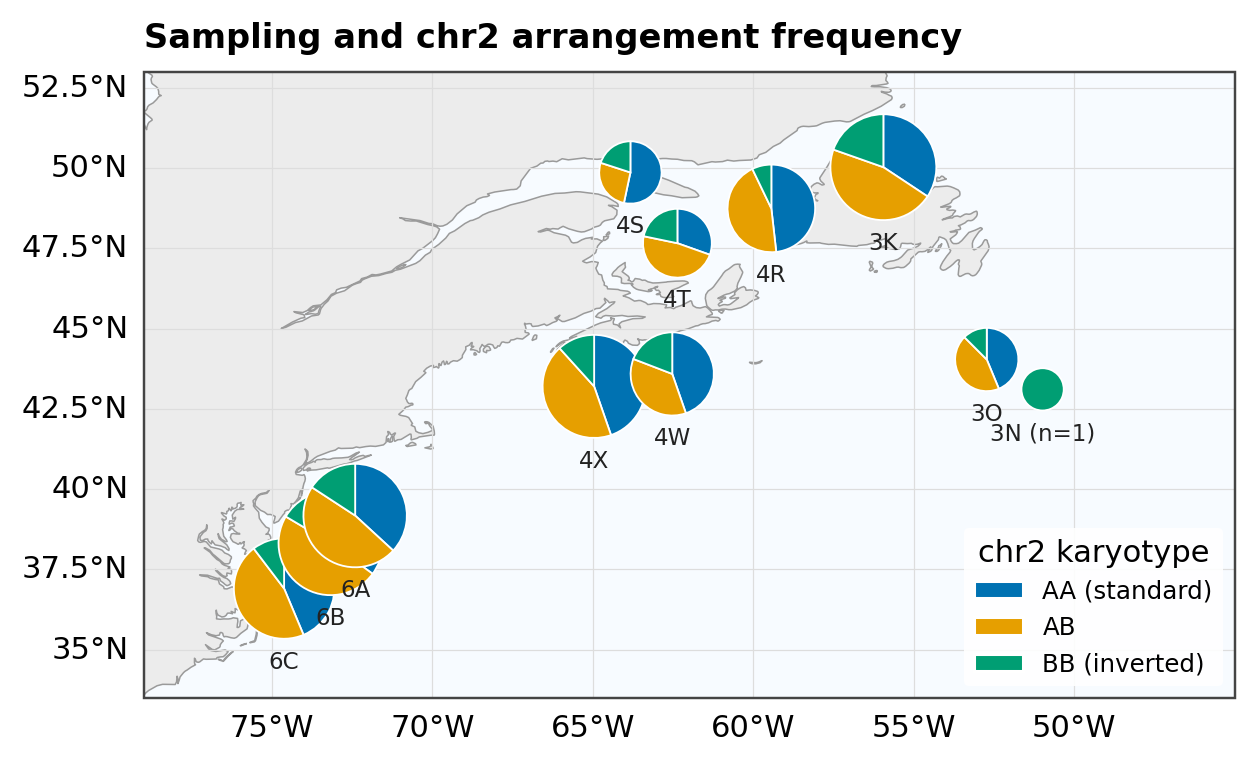
\includegraphics[width=.72\linewidth]{fig1_map.png}
  \caption{\textbf{Sampling and chromosome-2 arrangement frequency.} \illex{} sampled across eleven NAFO
    divisions ($\sim$37--50$^\circ$N); pies are placed at the mean sampling coordinates of each division and show
    the AA/AB/BB karyotype composition there (sized by $N$). The inverted (BB) frequency is non-clinal (0.29--0.46 across latitude), consistent with geographic $\Fst\approx0$: the inversion is not locally adaptive.}
  \label{fig:map}
\end{figure}

\begin{figure}[p]\centering
  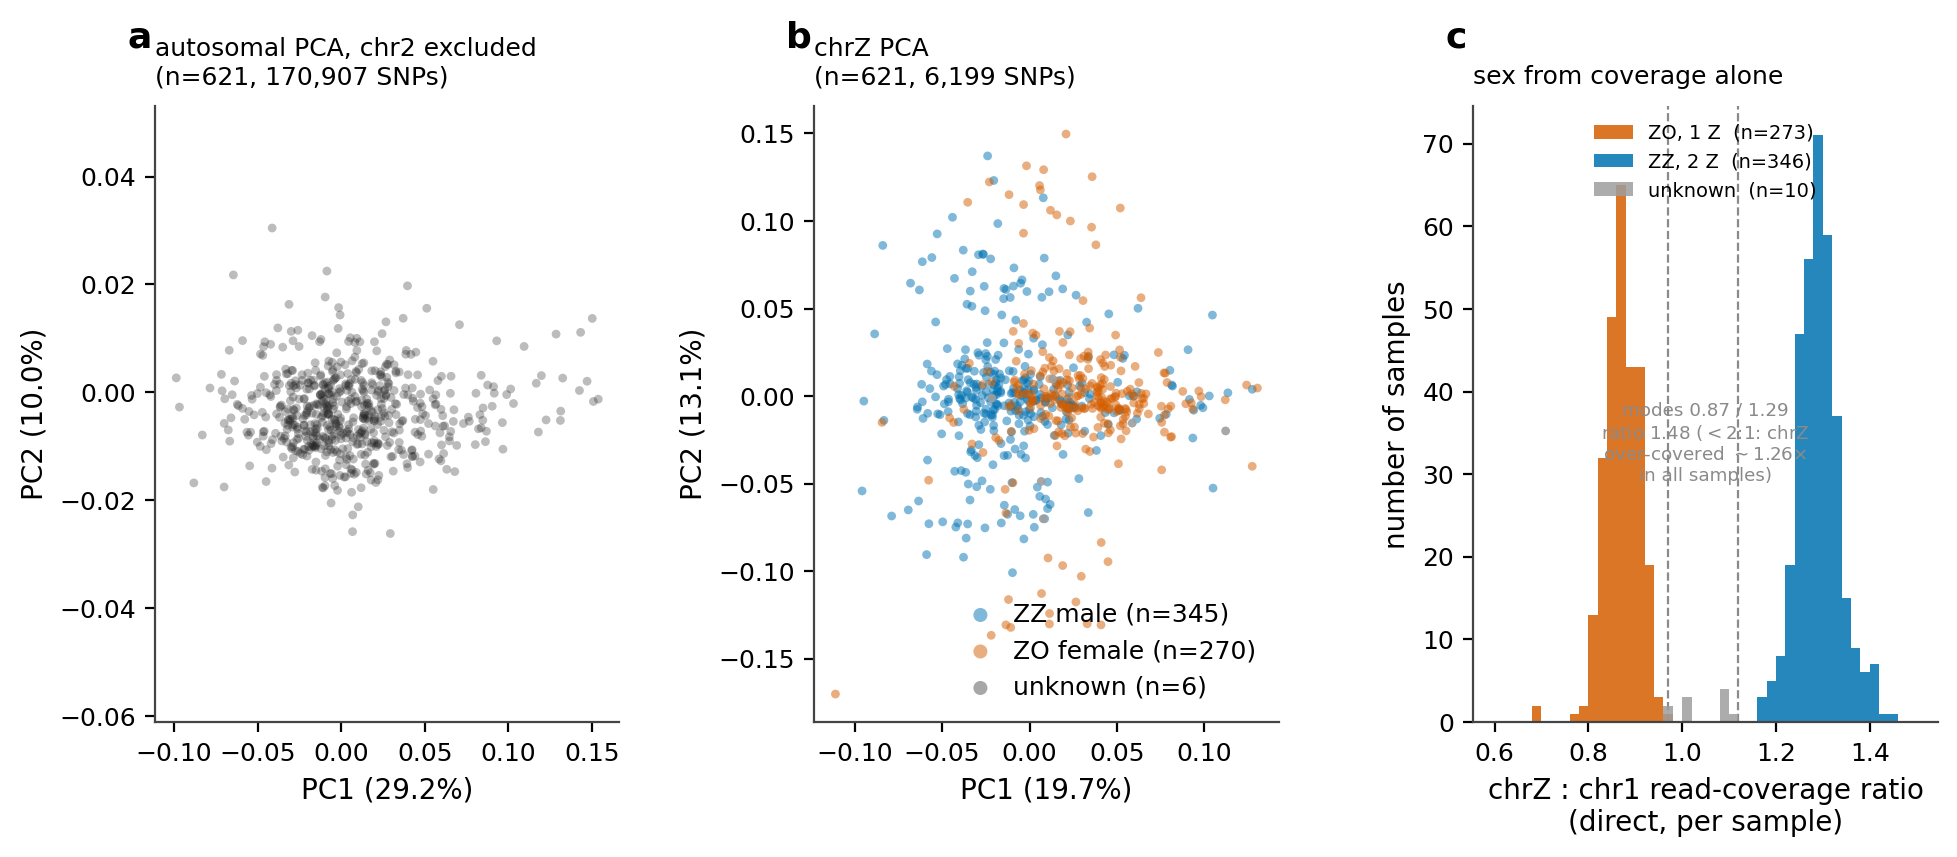
\includegraphics[width=\linewidth]{fig2_overview.png}
  \caption{\textbf{No population structure outside chr2, and the sex assignment} (consistent with the
    range-wide panmixia of \citealt{baker2025}). \textbf{(a)} Genome-wide autosomal PCA with chr2 excluded, a single undifferentiated cloud. \textbf{(b)} chrZ PCA (mild male/female separation). \textbf{(c)} chrZ:chr1
    read-coverage ratio by individual: ZZ males at $\sim$1.0 (two Z copies), ZO females near the single-copy
    expectation (there is no W); individuals in the ambiguous band are left unassigned. 342 males / 291
    females.}
  \label{fig:overview}
\end{figure}

\begin{figure}[p]\centering
  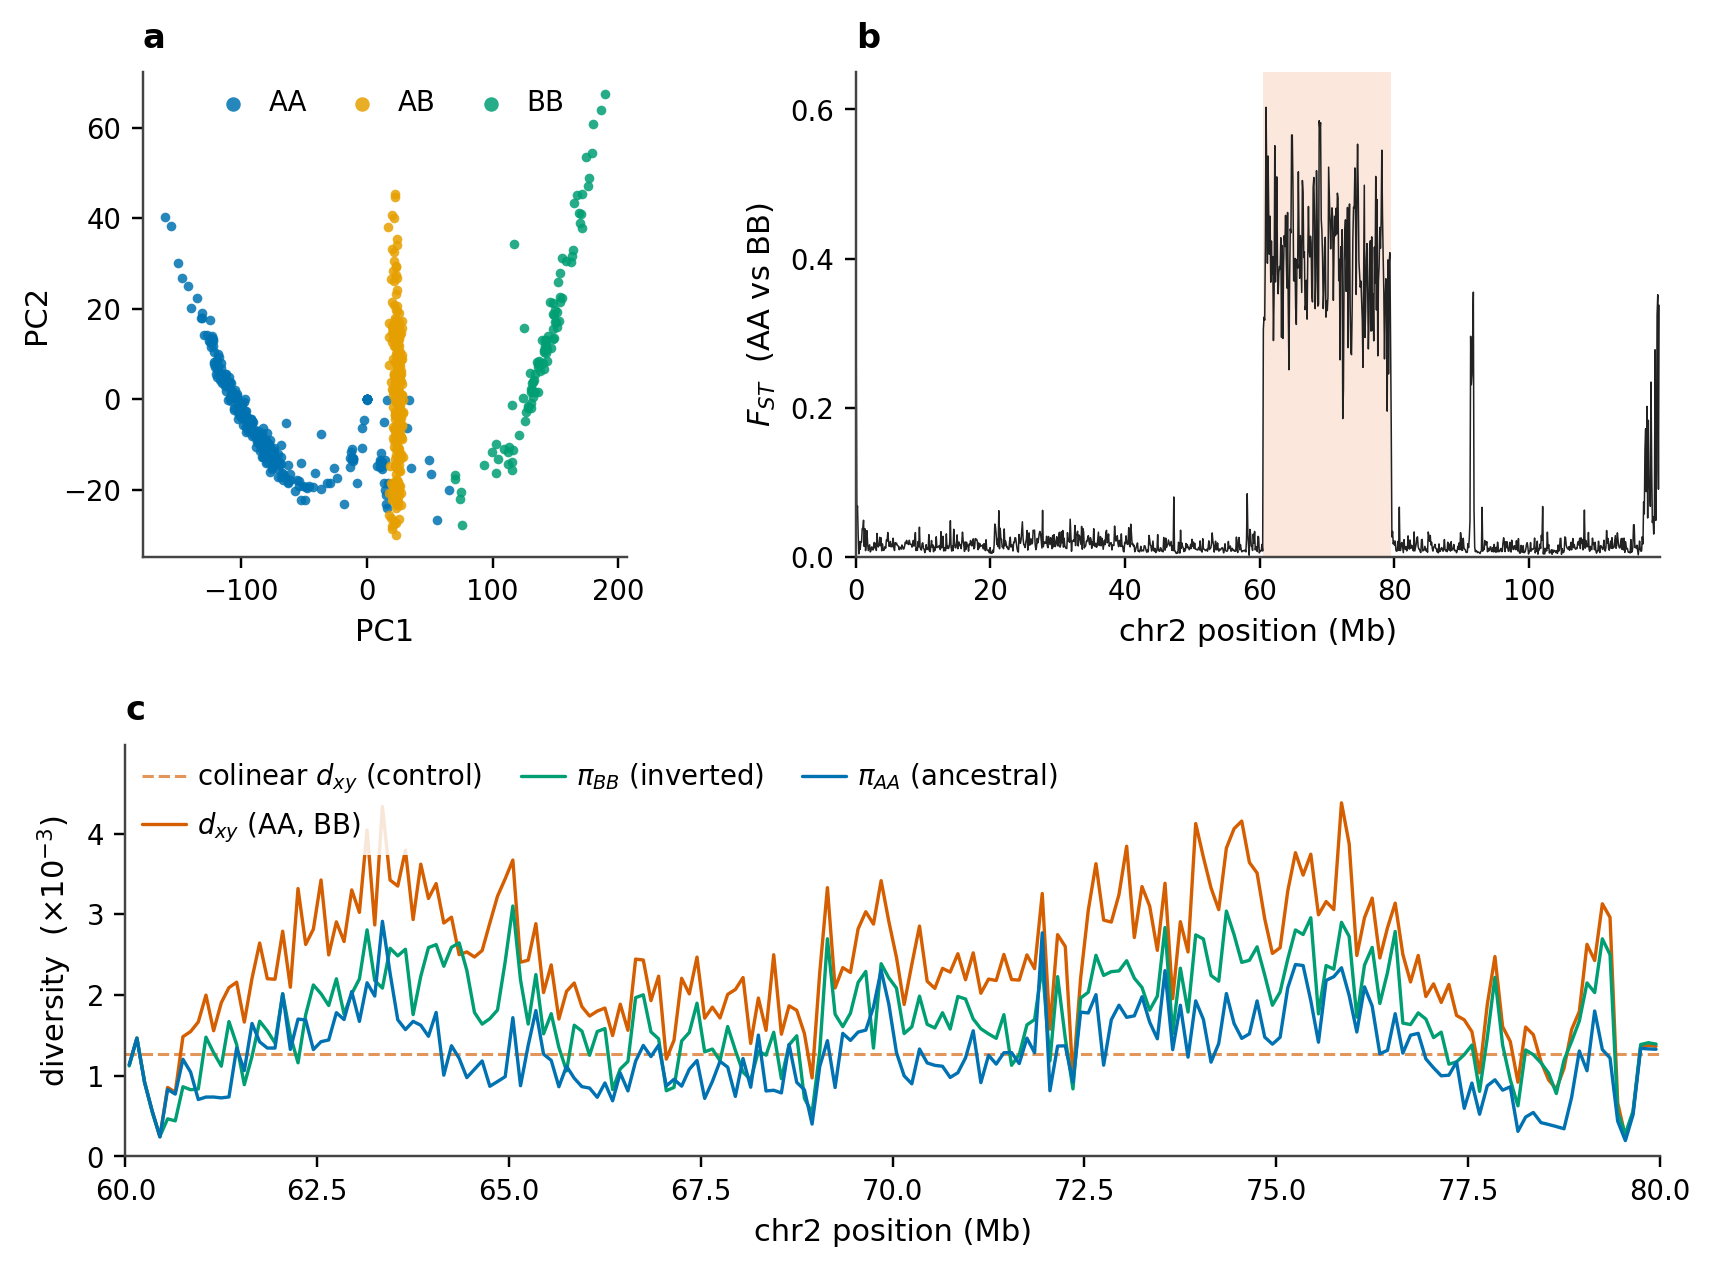
\includegraphics[width=\linewidth]{fig3_inversion.png}
  \caption{\textbf{The chromosome-2 inversion.} \textbf{(a)} chr2 PCA resolves three karyotype clusters
    (AA/AB/BB). \textbf{(b)} $\Fst$ between arrangements along chr2: the inversion (60.54--79.50~Mb, shaded) is the only differentiated region (median $\Fst=0.37$ vs 0.01 collinear; whole-chromosome view in
    Supplementary Fig.~S20). \textbf{(c)} Per-arrangement diversity across the inversion (shaded) and 20~Mb of
    collinear sequence on either side: inside the breakpoints the derived, inverted BB arrangement is more diverse than the ancestral AA ($\pi_I/\pi_S=1.36$) despite its lower frequency, and $\dxy$ exceeds both, the signature of an old, formerly common polymorphism; outside them the three curves
    collapse onto one another at the collinear $d_{xy}$ (dashed), as expected where the arrangements
    recombine freely.}
  \label{fig:inv}
\end{figure}

\begin{figure}[p]\centering
  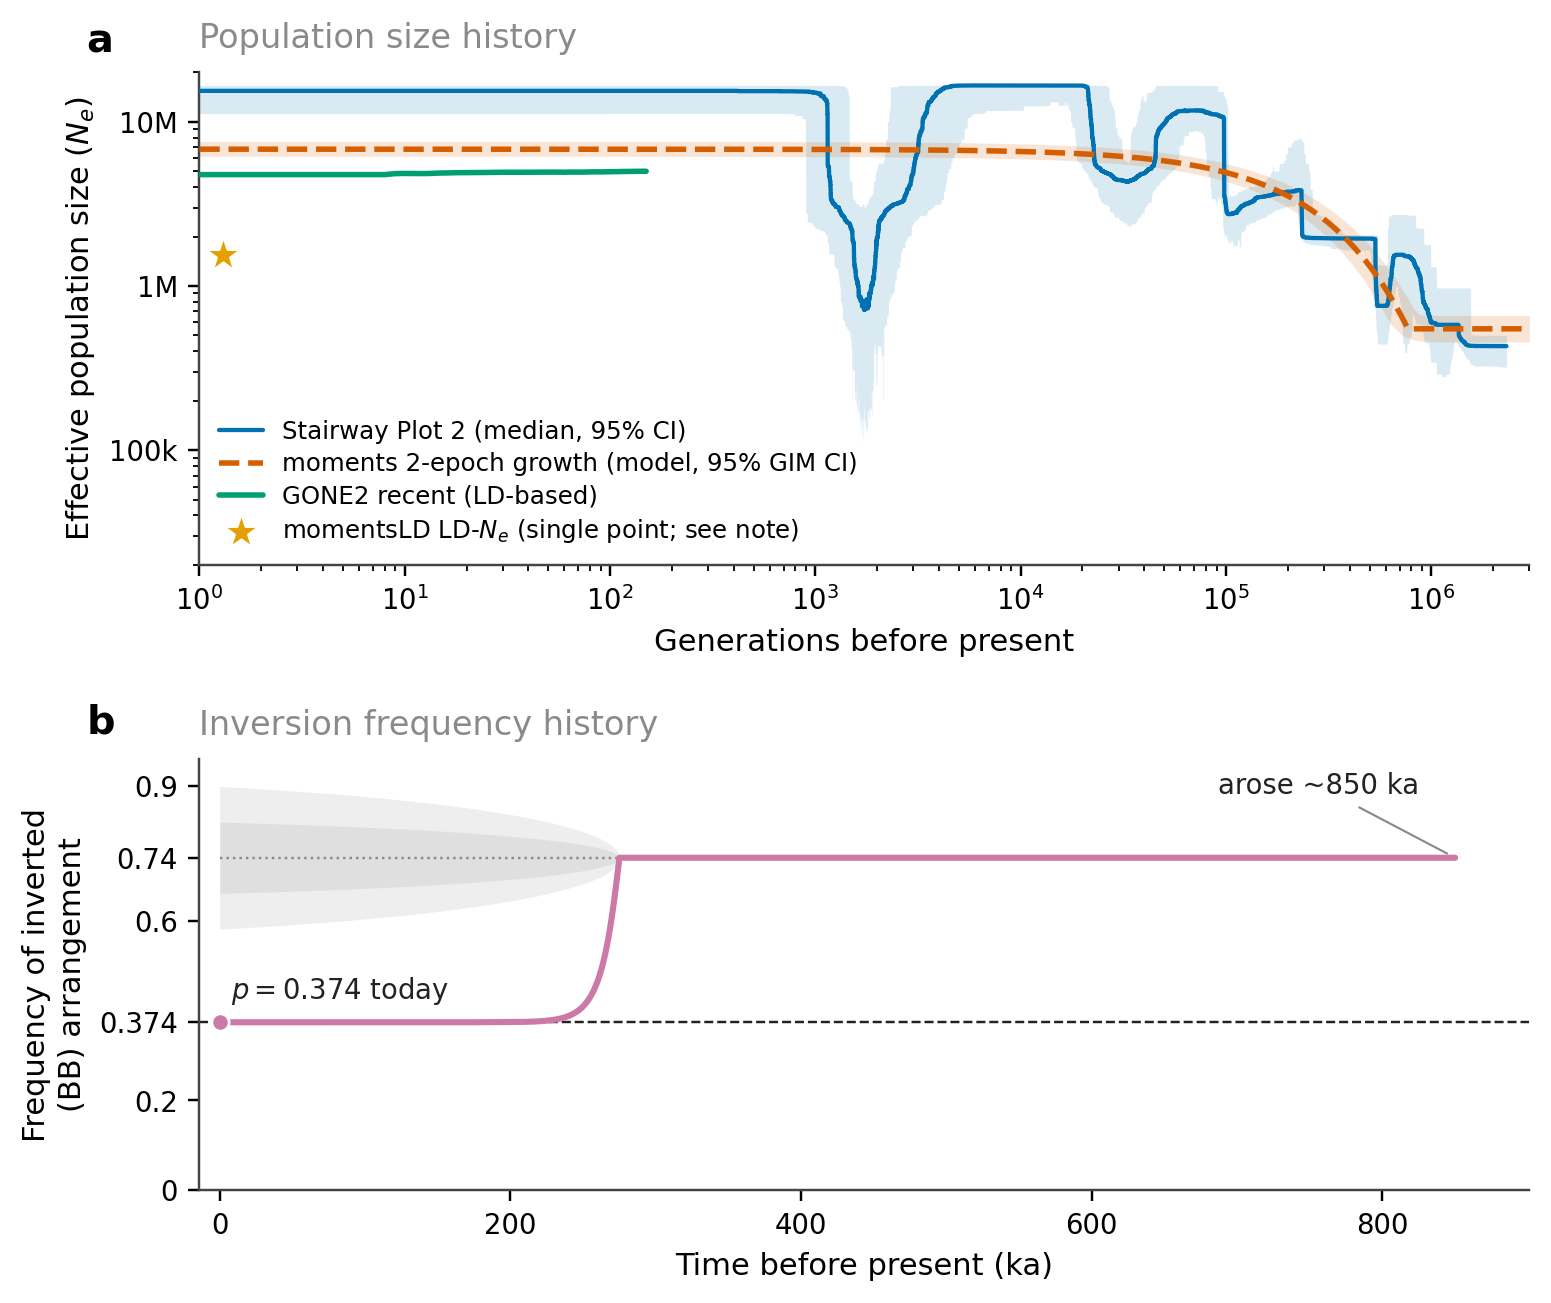
\includegraphics[width=\linewidth]{fig4_demography.png}
  \caption{\textbf{Demographic history and the inversion's frequency history.} \textbf{(a)} Effective
    population size over time: Stairway~Plot~2 (median $\pm$95\% CI), the moments 2-epoch growth model with
    its Godambe (GIM) 95\% parameter-CI envelope (expansion $12.4\times\pm9\%$, $T\approx770$~ky~$\pm16\%$),
    GONE2 for the recent past, and a single momentsLD LD-$\Ne$ point (rate-corrected; only the contemporary
    point is shown because its time-varying fit is non-identifiable). \textbf{(b)} Inversion trajectory fit
    with the barrier-aware coalescent simulator msinv: the derived (BB) arrangement arose $\sim$850~ka, coincident with the onset of expansion in (a), was held near $p\approx0.74$, and declined to 0.374;
    the neutral-drift envelope is shown for comparison. $\Delta\chi^{2}$ profiles locating the end and duration
    of the decline are in Supplementary Fig.~S14; the fall was recent and fast, excluding neutral drift-out.}
  \label{fig:demog}
\end{figure}

\begin{figure}[p]\centering
  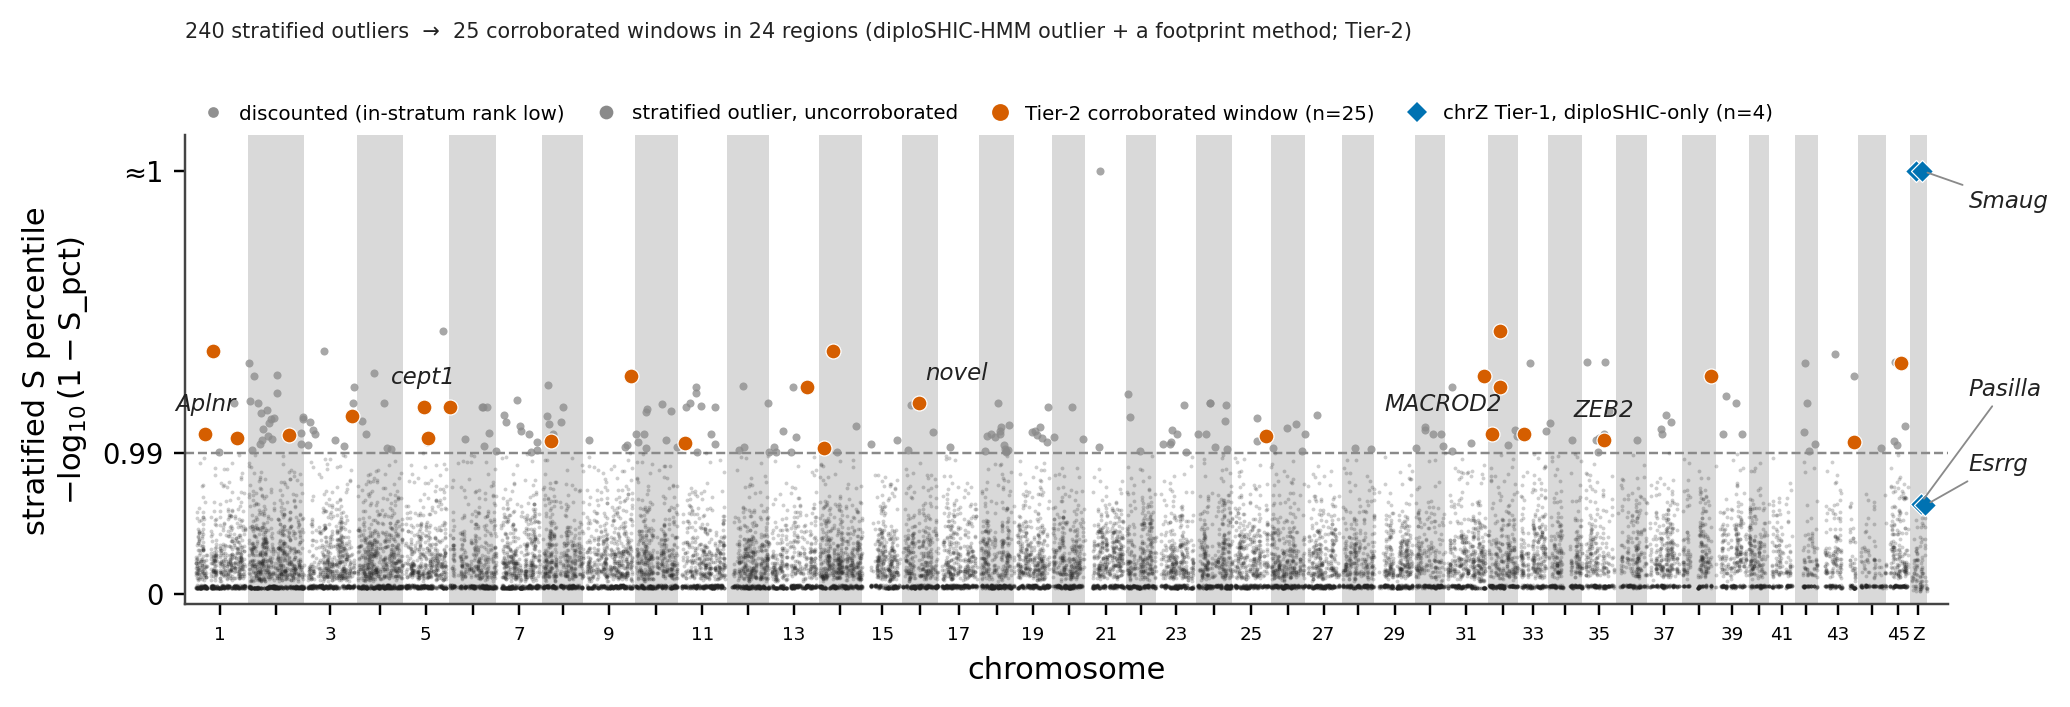
\includegraphics[width=\linewidth]{fig5_selection.png}
  \caption{\textbf{The genome-wide selective-sweep scan.} Sweep signal across the genome (chromosomes
    concatenated). The classifier reads the genome as pervasively linked-selected
    ($\sim$91\% linked-hard/soft; neutral $\sim$1\%; true hard/soft only a few percent), so raw diploS/HIC
    calls are filtered by cross-method concordance (a diploS/HIC-HMM outlier plus RAiSD or SweepFinder2) and a
    background-selection test; the corroborated, background-selection-robust candidates (35 windows across 34
    regions; highlighted) stand out above the discounted background, with key genes labelled. Chromosome-Z
    Tier-1 calls (diamonds; \textit{Pasilla}, \textit{Smaug}, \textit{Esrrg} labelled) are male-based and diploS/HIC-only (the footprint methods do not cover the Z), so they cannot enter the concordance
    filter. Chromosome~2 carries no concordant sweep. The full scan
    pipeline is shown in Supplementary Fig.~S8.}
  \label{fig:selection}
\end{figure}

\begin{figure}[p]\centering
  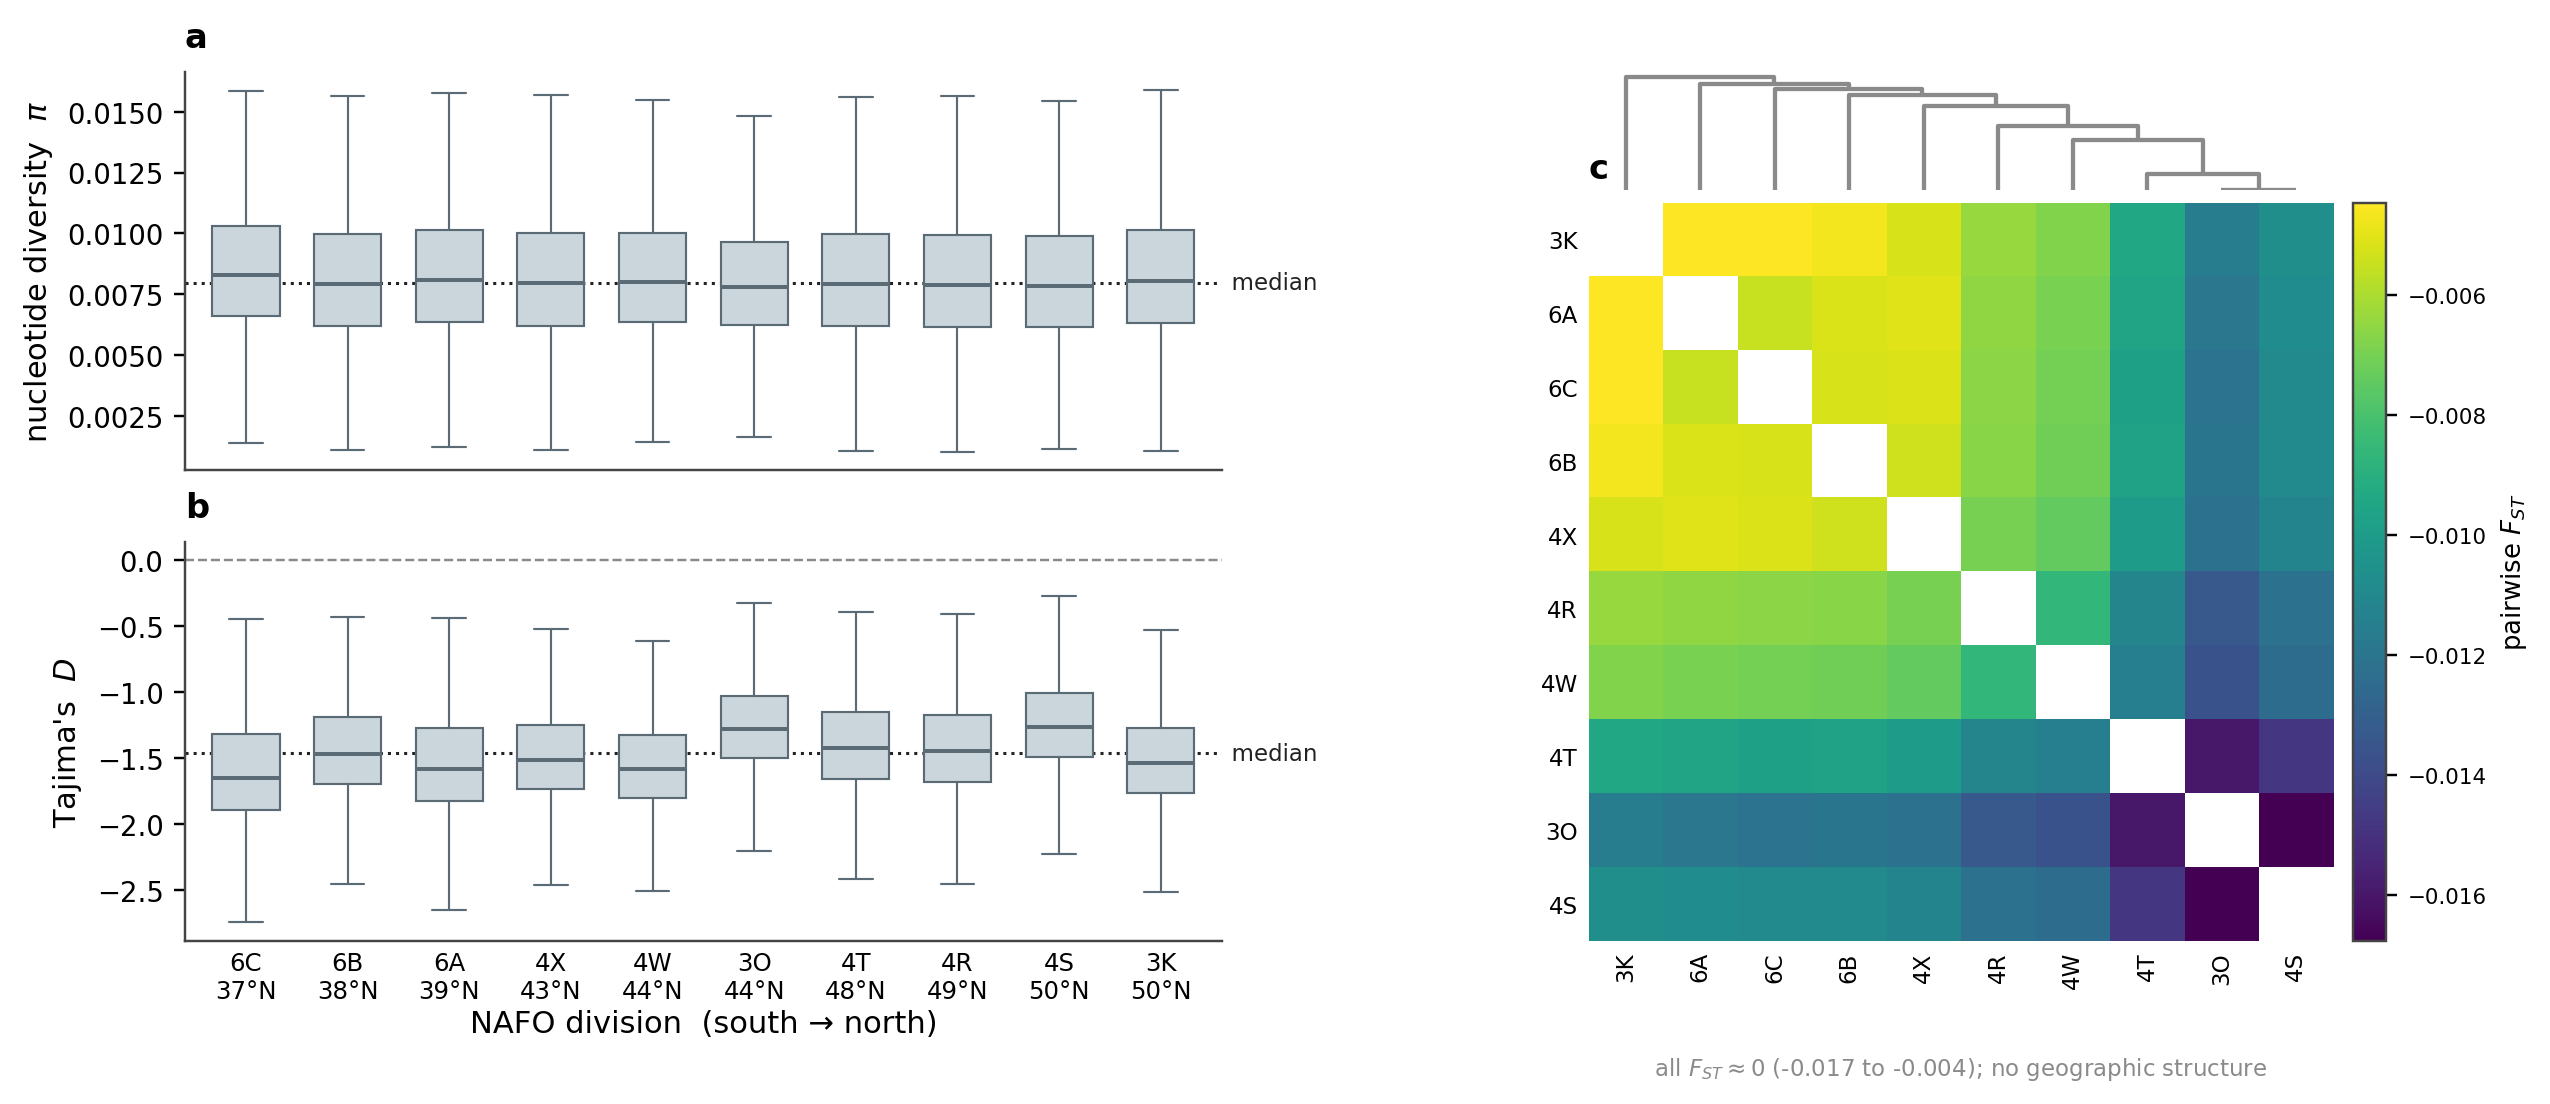
\includegraphics[width=\linewidth]{fig6_diversity.png}
  \caption{\textbf{Diversity is uniform and there is no geographic structure.} \textbf{(a)} Nucleotide
    diversity $\pi$ and \textbf{(b)} Tajima's $D$ per NAFO division (ten of the eleven sampled divisions;
    3N, with a single individual, cannot support per-population estimates), ordered south$\to$north: both are flat across latitude (no cline), and $D$ is negative in every population, the signature of strong
    expansion. \textbf{(c)} Pairwise $\Fst$ among divisions as a clustered heatmap with dendrogram: every
    value is $\approx0$ ($-0.017$ to $-0.004$) and the clustering follows sample size, not geography, i.e.\ no population structure. ($\pi$/$D$ estimated by ANGSD genotype likelihoods over all 45 autosomes plus the
    Z, large divisions subsampled to $n=25$; $\Fst$ genome-wide by pg\_gpu. Per-chromosome distributions:
    Supplementary Fig.~S9.)}
  \label{fig:diversity}
\end{figure}

% ------------------------------ TABLES -------------------------------
\begin{table}[t]\centering
  \caption{\textbf{Sample and whole-genome summary.} Diversity statistics are genome-wide from genotype
    likelihoods; karyotype counts and the inverted-arrangement frequency are for chromosome~2.}
  \label{tab:summary}
  \begin{tabular}{ll}
    \toprule
    Quantity & Value \\
    \midrule
    Species / callset            & \illex{}; \citet{baker2025} whole-genome \\
    Individuals (karyotyped)     & 633 \\
    Sex (chrZ coverage)          & 342 ZZ males / 291 ZO females \\
    Sampling                     & 11 NAFO divisions, $\sim$37--50$^\circ$N \\
    Geographic structure         & $\Fst\approx0$ (none outside chr2) \\
    Genome-wide $\pi$            & 0.0093 \\
    Genome-wide Tajima's $D$     & $-2.07$ ($-2.09$ in 50~kb windows) \\
    chr2 karyotypes (AA/AB/BB)   & 254 / 284 / 95 \\
    Inverted (BB) frequency      & 0.374 (0.29--0.46 across divisions, non-clinal) \\
    Karyotype $\Fst$(AA,BB)      & 0.365 \\
    \bottomrule
  \end{tabular}
\end{table}

\begin{table}[t]\centering
  \caption{\textbf{The chromosome-2 inversion} (corrected polarisation: I~$=$~BB inverted/derived,
    S~$=$~AA ancestral/standard).}
  \label{tab:inv}
  \begin{tabular}{ll}
    \toprule
    Quantity & Value \\
    \midrule
    Location (differentiated body) & chr2:60.54--79.50~Mb ($\sim$18.96~Mb) \\
    Karyotypes (AA/AB/BB)          & 254 / 284 / 95 (95.3\% confident) \\
    Inverted (BB) frequency $p$    & 0.374 \\
    Historical peak frequency      & $\sim$0.74 \\
    Karyotype $\Fst$(AA,BB)        & 0.365 (geographic $\Fst\approx0$) \\
    $\pi_I/\pi_S$ (I$=$BB)         & $1.356 \pm 0.048$ \\
    $\dxy/\pi_I$                   & $1.385 \pm 0.021$ \\
    Coalescent age $t_\mathrm{inv}$ & $\sim$850~ky ($\propto 1/\mu$, $\mu=3\times10^{-9}$) \\
    Decline                        & $0.74\to0.374$ over $\sim$50--100~ky, ending $\gtrsim$50--100~ka \\
    Selection on decline           & $\Ne s\sim10^{2}$--$10^{3}$ ($s\approx1.5\times10^{-4}$) \\
    Gene content                   & 89 gene models, 45 annotated; no GO enrichment ($p=0.51$) \\
    Fixed differences (AA vs BB)   & 3{,}513; 19 exonic, in 9 genes \\
    \bottomrule
  \end{tabular}
\end{table}

\begin{table}[t]\centering
  \caption{\textbf{Demographic model} (moments, folded SFS; validated by forward simulation).}
  \label{tab:demog}
  \begin{tabular}{ll}
    \toprule
    Parameter & Value \\
    \midrule
    Ancestral $\Ne$ (N\_REF)     & 547{,}928 \\
    Present $\Ne$ (N0)           & 6{,}808{,}096 \\
    Growth duration (T\_GROW)    & 769{,}519 generations \\
    Fold expansion               & $\sim$12$\times$ \\
    Genome-wide $\pi$            & 0.0093 \\
    Genome-wide Tajima's $D$     & $\approx-2$ (nearly all windows) \\
    Mutation rate $\mu$          & $3\times10^{-9}$ / bp / generation \\
    Recombination (autosomal)    & $\sim$0.21--0.24~cM/Mb (sex-averaged) \\
    \bottomrule
  \end{tabular}
\end{table}

\begin{table}[t]\centering
  \caption{\textbf{High-confidence selective-sweep candidates}, grouped by biological function and ordered by
    chromosome, including the Z-chromosome set. Autosomal rows are the 11 background-selection-robust
    candidates (of 34 concordant regions); Z rows (marked) are the fine-scale-confirmed sweeps from the
    males-only scan. Genes are cephalopod orthologs. Class: hard/soft sweep. Full machine-readable tables:
    Supplementary Table~S6.}
  \label{tab:sweep}
  \begin{tabular}{lll}
    \toprule
    Location & Gene / feature & Class \\
    \midrule
    \multicolumn{3}{l}{\itshape Neural, RNA-regulation \& development}\\
    chr35:39.0~Mb & \textit{ZEB2} (neural/EMT transcription factor)        & hard \\
    Z:20.8~Mb     & \textit{Pasilla}/Nova-1 (splicing regulator)          & hard (Z) \\
    Z:23.6~Mb     & \textit{Smaug}/samd4a (translational repressor)       & hard (Z) \\
    \multicolumn{3}{l}{\itshape Cardiovascular}\\
    chr1:20.3~Mb  & \textit{Aplnr} (apelin receptor)                      & hard \\
    \multicolumn{3}{l}{\itshape Genome-maintenance \& stress}\\
    chr32:9.3~Mb  & \textit{MACROD2} (DNA-damage response)                & soft \\
    \multicolumn{3}{l}{\itshape Membrane \& lipid}\\
    chr5:38.0~Mb  & \textit{cept1} (phospholipid synthesis)               & hard \\
    chr1:85.5~Mb  & ceramide phosphoethanolamine synthase\,$^{\dagger}$   & hard \\
    \multicolumn{3}{l}{\itshape Metabolism}\\
    chr25:65.0~Mb & \textit{GALT}\,$^{\dagger}$                           & soft \\
    \multicolumn{3}{l}{\itshape ECM \& adhesion}\\
    chr33:9.0~Mb  & \textit{Tinagl1}                                      & hard \\
    \multicolumn{3}{l}{\itshape Signalling}\\
    chr32:24.1~Mb & GPCR cluster                                          & hard \\
    Z:30.7~Mb     & \textit{Esrrg} (estrogen-related receptor)            & soft (Z) \\
    \multicolumn{3}{l}{\itshape Cephalopod-specific novelty}\\
    chr16:35.3~Mb & uncharacterised (\textit{Euprymna} family)            & hard \\
    \multicolumn{3}{l}{\itshape Lower confidence (TE-dense)}\\
    chr1:35.9~Mb  & transposable element\,$^{\ddagger}$                   & hard \\
    chr11:10.8~Mb & transposable element\,$^{\ddagger}$                   & hard \\
    \bottomrule
  \end{tabular}
  \\[2pt]
  {\footnotesize $^{\dagger}$ target reassigned by fine-scale localisation (annotation-recovered gene).
   $^{\ddagger}$ TE-dense region; deep-$\pi$/negative-$D$ may be a TE-insertion sweep or a repeat artifact.}
\end{table}

% =====================================================================
\clearpage
\bibliographystyle{plainnat}
\bibliography{references}

\end{document}
